\hypertarget{a00011}{
\section{Dokumentacja klasy ASS8.Klient.klientUpload}
\label{da/d45/a00011}\index{ASS8::Klient::klientUpload@{ASS8::Klient::klientUpload}}
}
Klasa zawiera dane do serializacji zapytania o wysyłanie pliku.  


Dziedziczy \hyperlink{a00007}{ASS8::Klient::klientBase}.

Diagram współpracy dla ASS8.Klient.klientUpload:\nopagebreak
\begin{figure}[H]
\begin{center}
\leavevmode
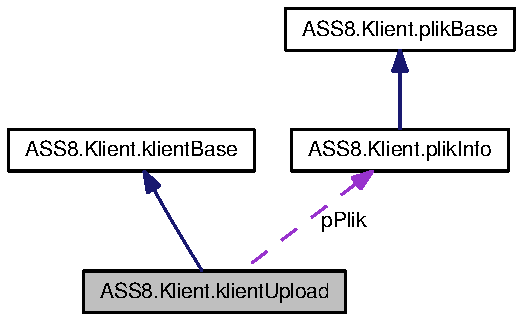
\includegraphics[width=287pt]{d7/da0/a00198}
\end{center}
\end{figure}
\subsection*{Metody publiczne}
\begin{CompactItemize}
\item 
\hyperlink{a00011_360231a3cc7ad8d86b5245eaeec18711}{klientUpload} ()
\item 
\hyperlink{a00011_8a61f3de65e9fe569185ad9a70c8865f}{klientUpload} (int id, int oper, string n, long d, int r, int dos, string h)
\end{CompactItemize}
\subsection*{Właściwości}
\begin{CompactItemize}
\item 
\hyperlink{a00018}{plikInfo} \hyperlink{a00011_768e461c6c80e2703893b7634d00146b}{plik}\hspace{0.3cm}{\tt  \mbox{[}get, set\mbox{]}}
\end{CompactItemize}
\subsection*{Atrybuty prywatne}
\begin{CompactItemize}
\item 
\hyperlink{a00018}{plikInfo} \hyperlink{a00011_b6779c02575a79c4964354a61dd9088f}{pPlik}
\end{CompactItemize}


\subsection{Opis szczegółowy}
Klasa zawiera dane do serializacji zapytania o wysyłanie pliku. 



Definicja w linii 280 pliku XmlRequestsClass.cs.

\subsection{Dokumentacja konstruktora i destruktora}
\hypertarget{a00011_360231a3cc7ad8d86b5245eaeec18711}{
\index{ASS8::Klient::klientUpload@{ASS8::Klient::klientUpload}!klientUpload@{klientUpload}}
\index{klientUpload@{klientUpload}!ASS8::Klient::klientUpload@{ASS8::Klient::klientUpload}}
\subsubsection[{klientUpload}]{\setlength{\rightskip}{0pt plus 5cm}ASS8.Klient.klientUpload.klientUpload ()}}
\label{da/d45/a00011_360231a3cc7ad8d86b5245eaeec18711}




Definicja w linii 283 pliku XmlRequestsClass.cs.\hypertarget{a00011_8a61f3de65e9fe569185ad9a70c8865f}{
\index{ASS8::Klient::klientUpload@{ASS8::Klient::klientUpload}!klientUpload@{klientUpload}}
\index{klientUpload@{klientUpload}!ASS8::Klient::klientUpload@{ASS8::Klient::klientUpload}}
\subsubsection[{klientUpload}]{\setlength{\rightskip}{0pt plus 5cm}ASS8.Klient.klientUpload.klientUpload (int {\em id}, \/  int {\em oper}, \/  string {\em n}, \/  long {\em d}, \/  int {\em r}, \/  int {\em dos}, \/  string {\em h})}}
\label{da/d45/a00011_8a61f3de65e9fe569185ad9a70c8865f}




Definicja w linii 286 pliku XmlRequestsClass.cs.

\subsection{Dokumentacja atrybutów składowych}
\hypertarget{a00011_b6779c02575a79c4964354a61dd9088f}{
\index{ASS8::Klient::klientUpload@{ASS8::Klient::klientUpload}!pPlik@{pPlik}}
\index{pPlik@{pPlik}!ASS8::Klient::klientUpload@{ASS8::Klient::klientUpload}}
\subsubsection[{pPlik}]{\setlength{\rightskip}{0pt plus 5cm}{\bf plikInfo} {\bf ASS8.Klient.klientUpload.pPlik}\hspace{0.3cm}{\tt  \mbox{[}private\mbox{]}}}}
\label{da/d45/a00011_b6779c02575a79c4964354a61dd9088f}




Definicja w linii 282 pliku XmlRequestsClass.cs.

\subsection{Dokumentacja właściwości}
\hypertarget{a00011_768e461c6c80e2703893b7634d00146b}{
\index{ASS8::Klient::klientUpload@{ASS8::Klient::klientUpload}!plik@{plik}}
\index{plik@{plik}!ASS8::Klient::klientUpload@{ASS8::Klient::klientUpload}}
\subsubsection[{plik}]{\setlength{\rightskip}{0pt plus 5cm}{\bf plikInfo} ASS8.Klient.klientUpload.plik\hspace{0.3cm}{\tt  \mbox{[}get, set\mbox{]}}}}
\label{da/d45/a00011_768e461c6c80e2703893b7634d00146b}




Definicja w linii 293 pliku XmlRequestsClass.cs.

Dokumentacja dla tej klasy została wygenerowana z pliku:\begin{CompactItemize}
\item 
\hyperlink{a00055}{XmlRequestsClass.cs}\end{CompactItemize}
